
Computer Performance is the amount of work accomplished by a computer system. Computer software performance, particularly software application response time, is an aspect of software quality that is important in human–computer interactions. Depending on the context, high computer performance may involve one or more of the following:
\begin{itemize}
\item Short response time for a given piece of work
\item High throughput (rate of processing work)
\item Low utilization of computing resource(s)
\item High availability of the computing system or application
\item Fast (or highly compact) data compression and decompression
\item High bandwidth
\item Short data transmission time
\end{itemize}

Memory Hierarchy is important for Performance Enhancement as it ensures that maximum elements can be processed with minimum penalty of computer cycles.
\begin{figure}[ht]
\centering
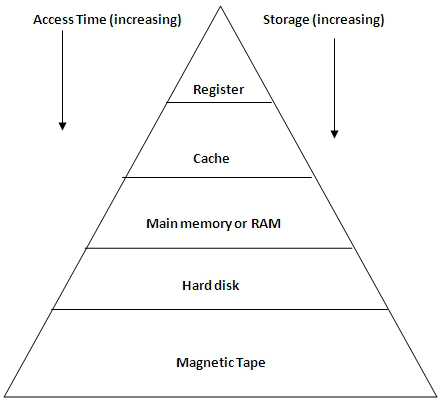
\includegraphics[scale=0.2]{images/perf.png}
\caption{Performance Enhancement}
\end{figure}
In computer science, locality of reference, also known as the principle of locality, is a term for the phenomenon in which the same values, or related storage locations, are frequently accessed, depending on the memory access pattern. There are two basic types of reference locality – temporal and spatial locality. Temporal locality refers to the reuse of specific data, and/or resources, within a relatively small time duration. Spatial locality refers to the use of data elements within relatively close storage locations. Sequential locality, a special case of spatial locality, occurs when data elements are arranged and accessed linearly, such as, traversing the elements in a one-dimensional array.
